\chapter{Introduction to Nepali Language Model}
\section{Abstract}
Language modeling (LM) is the use of various statistical and probabilistic techniques to determine the probability of a given sequence of words occurring in a sentence. Language models analyze bodies of text data to provide a basis for their word predictions. They are used in natural language processing (NLP) applications, particularly ones that generate text as an output. Some of these applications include , machine translation and question answering.

Some common statistical language model are:

\subsection{N-gram} 
N-grams are a relatively simple approach to language models. They create a probability distribution for a sequence of n The n can be any number, and defines the size of the "gram", or sequence of words being assigned a probability. For example, if n = 5, a gram might look like this: "can you please call me." The model then assigns probabilities using sequences of n size. Basically, n can be thought of as the amount of context the model is told to consider. Some types of n-grams are unigrams, bigrams, trigrams and so on.

\subsection{Continuous Space}
This type of model represents words as a non-linear combination of weights in a neural network. The process of assigning a weight to a word is also known as word embedding. This type becomes especially useful as data sets get increasingly large, because larger datasets often include more unique words. The presence of a lot of unique or rarely used words can cause problems for linear model like an n-gram. This is because the amount of possible word sequences increases, and the patterns that inform results become weaker. By weighting words in a non-linear, distributed way, this model can "learn" to approximate words and therefore not be misled by any unknown values. Its "understanding" of a given word is not as tightly tethered to the immediate surrounding words as it is in n-gram models.

\textbf{Keywords : } Transformers, LSTMs, Word2Vec, Attention, Tokenization

\begin{figure}[H]
    \centering
    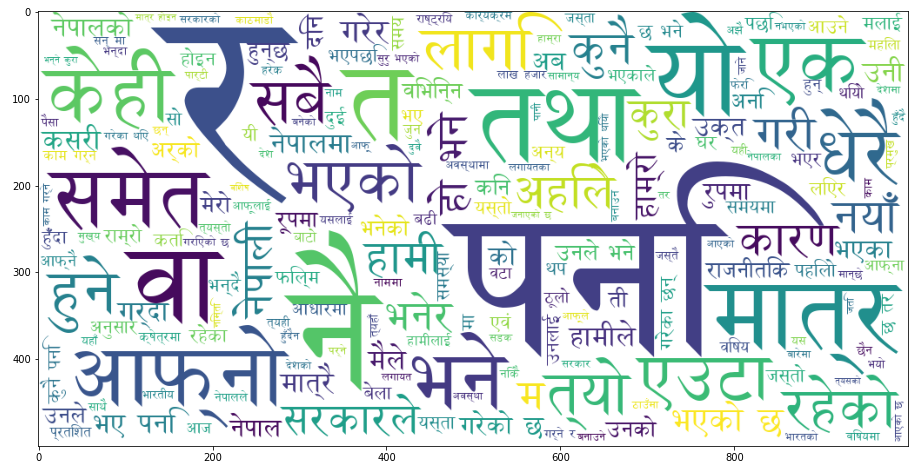
\includegraphics[scale = 0.5]{word_cloud.png}
    \caption{Nepali Word Cloud}
    \label{fig:Nepali Word Cloud}
\end{figure}

\section{Problem Statement}
\begin{enumerate}
    \item Nepali Language is rich in vocabulary and it is difficult to choose the best possible vocab.
    \item Spelling correction for nepali language available today are based on dictionary rather than contextual meaning of the sentence.
    \item There is no proper development of various NLP tasks like text generation, text summarization, image captioning, text to speech, etc. due to lack of reliable nepali language model
\end{enumerate}

\section{Objectives}
\begin{enumerate}
    \item To develop nepali language model for text generation.
    \item Use the nepali language model to develop the spelling correction based on contextual meaning.
\end{enumerate}


\section{Expected Outcome}
For language generation model, after user input some text, language generation model should suggest next words as shown below.

\begin{figure}[H]
    \centering
    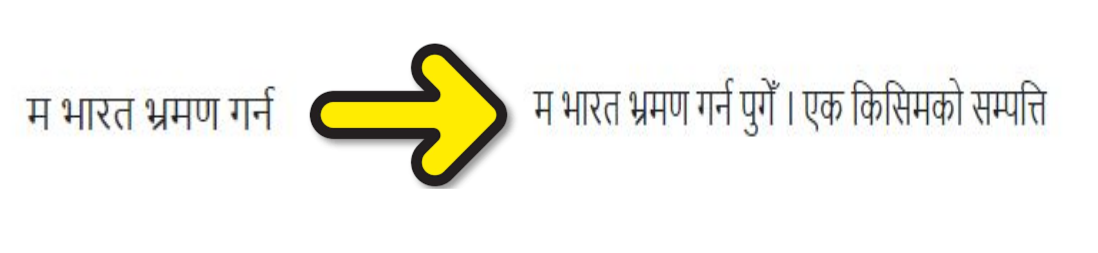
\includegraphics[scale = 0.35]{text_generation.png}
    \caption{Nepali Text Generation}
    \label{fig:Nepali Text Generation}
\end{figure}

Similarly, for the spelling correction model, the model should be able to correct word based on contextual meaning as shown below.

\begin{figure}[H]
    \centering
    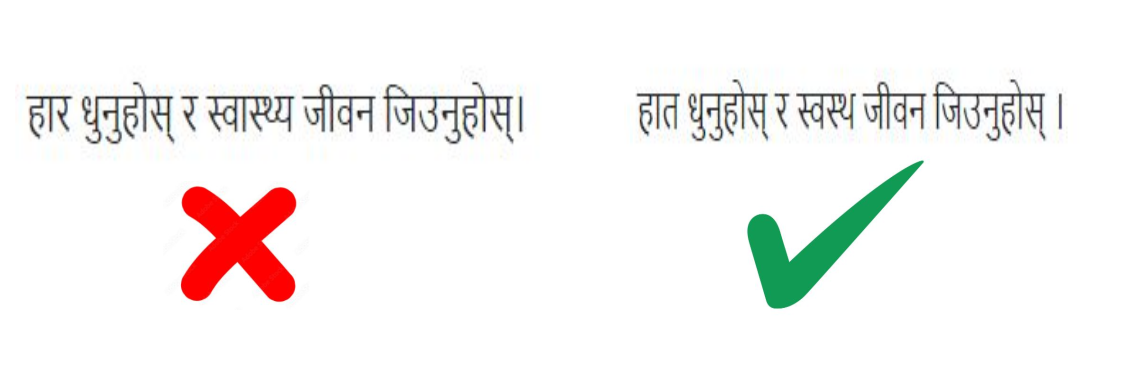
\includegraphics[scale = 0.35]{spelling_correction.png}
    \caption{Nepali Spelling Correction based on contextual meaning}
    \label{fig:Nepali Spelling Correction}
\end{figure}